\chapter{GENOME, TRANSCRIPTOME, AND METHYLOME SEQUENCING OF A PRIMITIVELY EUSOCIAL WASP REVEAL A GREATLY REDUCED DNA METHYLATION SYSTEM IN A SOCIAL INSECT}

A manuscript published in \textit{Molecular Ecology}.
\textbf{Supporting Information (SI)} available online: \href{http://dx.doi.org/10.1111/mec.13578}{doi:10.1111/mec.13578}.

\noindent\hfil\rule{0.5\textwidth}{.4pt}\hfil

Standage DS, Berens AJ, Glastad KM, Severin AJ, Brendel VP, Toth AL

\section{Abstract}

Comparative genomics of social insects has been intensely pursued in
recent years with the goal of providing insights into the evolution of
social behavior and its underlying genomic and epigenomic basis.
However, the comparative approach has been hampered by a paucity of data
on some of the most informative social forms (e.g. incipiently and
primitively social) and taxa (especially members of the paper wasp
family Vespidae) for studying social evolution. Here we provide a draft
genome of the primitively eusocial model insect \textit{Polistes
dominula}, accompanied by analysis of caste-related transcriptome and
methylome sequence data for adult queens and workers. \textit{P. dominula}
possesses a fairly typical hymenopteran genome, but shows very low
genome-wide GC content and some evidence of reduced genome size. We
found numerous caste-related differences in gene expression, with
evidence that both conserved and novel genes are related to caste
differences. Most strikingly, these --omics data reveal a major
reduction in one of the major epigenetic mechanisms that has been
previously suggested to be important for caste differences in social
insects: DNA methylation. Along with a conspicuous loss of a key gene
associated with environmentally responsive DNA methylation (the de novo
DNA methyltransferase \textit{Dnmt3}), these wasps have greatly reduced
genome-wide methylation to almost zero. In addition to providing a
valuable resource for comparative analysis of social insect evolution,
our integrative --omics data for this important behavioral and
evolutionary model system call into question the general importance of
DNA methylation in caste differences and evolution in social insects.

\section{Introduction}

The rapidly increasing availability of genomic resources for
non-traditional model organisms with well-developed social behavior has
incited great interest in the genomic basis of complex social life, or
sociogenomics \cite{Robinson2005}. Sociogenomic studies on a variety of species, from rodents
to fish to insects, have provided a wealth of information about the
transcriptomic and genomic characters associated with different forms of
derived social behavior, from affiliative behavior, to aggression, to
division of labor within animal societies
\cite{Robinson2008}. To
date, however, these studies have focused on relatively few species
separately, and current data have not allowed a comprehensive
comparative and phylogenetic approach to understanding the genomic
changes that accompany the evolution of sociality. As advances in
sequencing technology have greatly facilitated the generation of
genome-scale data for emerging model species \cite{Rokas2009}, it is an
exciting time to seek integration of genomic, transcriptomic, and
epigenomic data from species at key transitional points in the evolution
of sociality from solitary behavior.

The eusocial insects are one of the most important sociogenomic model
groups, comprising a diverse and ecologically successful group of
animals with a highly derived form of social behavior characterized by
the presence of reproductive and non-reproductive castes \cite{Superorganism}.
Eusocial insects are excellent models for understanding the evolution of
complexity as the switch from solitary to eusocial life marks one of the
major transitions in evolution due to the shift from individual
selection to colony level selection
\cite{MaynardSmith1995}.
Currently, published genome sequences are available for three parasitic
\textit{Nasonia} wasps \cite{Werren2010}, which provide a solitary outgroup for all of the
social Hymenoptera species, and 20 eusocial insect genomes---ten bees
\cite{KapheimTenBee,Kocher2013,Sadd2015,HoneybeeGenome} and
nine ants \cite{Bonasio2010,Nygaard2011,Oxley2014,LhumGenome,PbarGenome,AcepGenome,SinvGenome}, and very
recently, one paper wasp \cite{PcanGenome}. These studies provide important baseline data on
genomic characters associated with eusociality.

Importantly however, prior comparative sociogenomic analyses within the
social insects have suffered from two major deficits. First, there have
been relatively scant genomic resources available for one of the three
major hymenopteran eusocial lineages, the paper wasp family Vespidae
(\textbf{Figure \ref{Fig:Pdom1}A}). Although social wasps, bees, and ants evolved from
a common ancestor over 100 million years ago, these societies have
independently evolved many convergent features, including the presence
of female castes in the form of queens and workers. Second, there have
been relatively few genome sequences available for species in key
transitional stages between solitary and eusocial forms (notably, there
has been a large recent advance in this area
(\protect\hyperlink{ux5fENREFux5f24}{Kapheim \textit{et al.} 2015};
\protect\hyperlink{ux5fENREFux5f25}{Kocher \textit{et al.} 2013};
\protect\hyperlink{ux5fENREFux5f43}{Patalano \textit{et al.} 2015};
\protect\hyperlink{ux5fENREFux5f51}{Sadd \textit{et al.} 2015})). Here, we
expand the potential for comparative genomics of eusocial Hymenoptera by
describing the first complete genome sequence of \textit{Polistes
dominula}, a behavioral model species within the family Vespidae that
exhibits an intermediate form of social behavior, making it highly
informative for studying the evolution of sociality
(\protect\hyperlink{ux5fENREFux5f21}{Jandt \& Toth 2015}).

\textit{Polistes} wasps form small ``primitively eusocial'' societies
containing queens and altruistic workers, but unlike honey bees, their
colonies are characterized by prominent conflict over reproduction
(\protect\hyperlink{ux5fENREFux5f41}{Pardi 1948}). Queens and workers
engage in dominance interactions and there is constant competition
between females for reproductive opportunities. In addition,
\textit{Polistes} have small colonies with a relatively small number of
individuals, and colonies are started anew annually by founding queens
(\protect\hyperlink{ux5fENREFux5f46}{Reeve 1991}). These characteristics
have made \textit{Polistes} one of the main systems for testing hypotheses
about the evolution of altruistic behavior
(\protect\hyperlink{ux5fENREFux5f71}{West-Eberhard 1996}). For example,
studies of cooperation and conflict in small groups of \textit{Polistes}
wasps have provided some key tests of how genetic relatedness can
facilitate cooperation (\protect\hyperlink{ux5fENREFux5f17}{Hamilton
1964}). In addition, observations of \textit{Polistes} behavior led to new
hypotheses about the evolution of altruistic behavior from maternal
behavior (\protect\hyperlink{ux5fENREFux5f71}{West-Eberhard 1996}),
which have derived some support from transcriptomic studies
(\protect\hyperlink{ux5fENREFux5f62}{Toth \textit{et al.} 2010};
\protect\hyperlink{ux5fENREFux5f63}{Toth \textit{et al.} 2007}). A genome
sequence for \textit{Polistes dominula}, the best-studied member of the
model genus \textit{Polistes,} greatly enhances our power to study the
genetics of social behavior \textit{via} comparative genomic and
transcriptomic analyses, allowing for the identification of protein
coding changes, regulatory regions, and epigenetic modifications
associated with sociality. To facilitate future comparative analyses, we
provide a high quality draft \textit{P. dominula} genome and describe
informative features of this genome in reference to other previously
published bee, ant, and \textit{Nasonia} wasp genomes. Our genome sequence
was derived from an invasive population (from Pennsylvania, USA) of
\textit{Polistes dominula}, a temperate species that is native to Europe.
Our genome represents the second published paper wasp genome, the first
being the very recently published genome of the Neotropical paper wasp
\textit{Polistes canadensis} (\protect\hyperlink{ux5fENREFux5f43}{Patalano
\textit{et al.} 2015}). Although both species are primitively eusocial,
they are not closely related (split between Old and New World
\textit{Polistes} at 10-80 million years
(\protect\hyperlink{ux5fENREFux5f9}{Ezenwa \textit{et al.} 1998})) and
have several differences in their ecology and social biology. Thus, we
provide comparisons between these congeners, confirming many conserved
\textit{Polistes} genome characteristics but also highlighting some
conspicuous differences between the two paper wasp genomes.

One of the most active recent areas of research in insect sociogenomics
centers on the role of epigenetics in the regulation and evolution of
eusociality. Recent studies suggest epigenetic modifications to DNA are
ubiquitous within the social Hymenoptera
(\protect\hyperlink{ux5fENREFux5f26}{Kronforst \textit{et al.} 2008};
\protect\hyperlink{ux5fENREFux5f67}{Weiner \textit{et al.} 2013}), and
furthermore, various authors have suggested that differential DNA
methylation during larval development contributes to caste differential
gene expression and alternative splicing
(\protect\hyperlink{ux5fENREFux5f32}{Li-Byarlay \textit{et al.} 2013};
\protect\hyperlink{ux5fENREFux5f33}{Lyko \textit{et al.} 2010}), and
differences in caste-related phenotypes
(\protect\hyperlink{ux5fENREFux5f28}{Kucharski \textit{et al.} 2008}) in
both honey bees and ants. We previously hypothesized that DNA
methylation might also be important for caste differential expression
and behavioral and physiological caste differences in primitively
eusocial species such as \textit{Polistes dominula}
(\protect\hyperlink{ux5fENREFux5f67}{Weiner \textit{et al.} 2013};
\protect\hyperlink{ux5fENREFux5f68}{Weiner \& Toth 2012}). However,
recent studies suggest DNA methylation may be less important for
primitively eusocial species, including \textit{Polistes canadensis}
(\protect\hyperlink{ux5fENREFux5f24}{Kapheim \textit{et al.} 2015};
\protect\hyperlink{ux5fENREFux5f43}{Patalano \textit{et al.}
2015})\textit{.} Therefore, we looked for evidence of a functional DNA
methylation system by investigating the presence of a full complement of
DNA methylation enzymes in the \textit{Polistes dominula} genome. In
addition, we performed RNA-sequencing and whole genome bisulfite
sequencing (methylome sequencing) on a set of adult queen and worker
samples in order to examine caste-associated differential expression and
DNA methylation in the \textit{Polistes dominula} genome. These
experiments provide a valuable point of comparison to other social
insects for assessing whether DNA methylation is a shared, general
mechanism related to sociality in insects.

\section{Materials and Methods}

Detailed protocols are provided in \textbf{SI Materials and Methods}.

\subsection{Sample collection and sequencing.} Five Illumina paired-end
whole genome shotgun libraries were prepared from a single pupal male
collected from an invasive population in State College, Pennsylvania.
The libraries, ranging in insert size from \textless{}200bp to 8Kbp (see
\textbf{Table S1}), were sequenced on the Illumina HiSeq 2000 platform.

Same-nest pairs of six adult workers and six egg-laying adult queens and
from six different colonies were collected for transcriptome and
methylome sequencing; these twelve individuals were from the same State
College, Pennsylvania population as the pupal male used for genome
sequencing. The head of each adult was cut in half, with RNA extracted
from one half for transcriptome sequencing and DNA extracted from the
other half for methylome sequencing.

\subsection{Genome assembly and annotation}. Five whole genome shotgun
libraries were assembled using the AllPaths-LG genome assembler
(\protect\hyperlink{ux5fENREFux5f14}{Gnerre \textit{et al.} 2011}), with
the smallest library designated as the \textit{fragment library} and the
other four libraries designated as \textit{jumping libraries}. The
assembled scaffolds were then screened for repetitive DNA, masked, and
annotated by the MAKER pipeline
(\protect\hyperlink{ux5fENREFux5f7}{Cantarel \textit{et al.} 2008}). The
annotation workflow incorporated evidence from spliced alignments of
transcripts from three \textit{Polistes} species, spliced alignments of
reference proteins from \textit{Apis mellifera} and \textit{Drosophila
melanogaster}, gene models produced by three \textit{ab initio} gene
predictors, and manual gene annotations contributed \textit{via} the
PdomGDB genome browser's community annotation portal.

\subsection{Transcriptome assembly and annotation}. Twelve Illumina
paired-end RNA-Seq libraries were assembled using the Trinity assembler
(\protect\hyperlink{ux5fENREFux5f15}{Grabherr \textit{et al.} 2011}) with
the -\/-CuffFly algorithm and the -\/-jaccard\_clip setting enabled.
Assembled transcripts were then post-processed to discard contaminants,
split transcript chimeras, and annotate transcript functions by
similarity to known proteins and miRNAs. Two previously published
\textit{Polistes} transcriptomes
(\protect\hyperlink{ux5fENREFux5f3}{Berens \textit{et al.} 2015b};
\protect\hyperlink{ux5fENREFux5f10}{Ferreira \textit{et al.} 2013}) were
processed with the same procedure.

\subsection{Differential expression analysis}. Twelve Illumina paired-end
RNA-Seq libraries, six from queens and six from workers, were sequenced
and reads were mapped individually to the genome using Bowtie
(\protect\hyperlink{ux5fENREFux5f29}{Langmead \textit{et al.} 2009}).
Preliminary examination of the alignments revealed an extremely wide
dynamic range of expression values (\textless{}10 reads to millions of
reads mapped per replicate) and in some cases considerable variation
between replicates. To account for these observations we discarded loci
with too many or too few reads mapped (normalized by sequence length) or
with a high coefficient of variation.

Expression was quantified using RSEM
(\protect\hyperlink{ux5fENREFux5f31}{Li \& Dewey 2011}), and the EBSeq
package (\protect\hyperlink{ux5fENREFux5f30}{Leng \textit{et al.} 2013})
was used for identifying loci with caste differential expression at a
false discovery rate of \textless{} 0.05. A complete description of the
number of raw reads, data filtering procedure, and software parameters
used is available in \textbf{SI Methods and Results}.

\subsection{Methylome analysis}. Two DNA samples (one pooled sample from
workers and one pooled sample from queens, derived from the same six
individuals used for transcriptome sequencing) were subjected to
bisulfite treatment, and each sample was used to generate separate
Illumina libraries for sequencing. The Bismark software
(\protect\hyperlink{ux5fENREFux5f27}{Krueger \& Andrews 2011}) was used
for read mapping and methylation calls. Highly supported methylation
sites were determined as sites with significant number of methylation
calls based on a binomial probability model with Bonferroni correction
at the 1\% significance level (assuming a 99.5\% conversion rate in the
treatment). We also reanalyzed existing datasets from from
\textit{Polistes canadensis} (\protect\hyperlink{ux5fENREFux5f43}{Patalano
\textit{et al.} 2015}), honey bees
(\protect\hyperlink{ux5fENREFux5f33}{Lyko \textit{et al.} 2010}), the ants
\textit{Harpegnathos saltator} and \textit{Camponotus floridanus}
(\protect\hyperlink{ux5fENREFux5f4}{Bonasio \textit{et al.} 2012}), and
the parasitoid wasp \textit{Nasonia vitripennis}
(\protect\hyperlink{ux5fENREFux5f65}{Wang \textit{et al.} 2013}) in order
to compare our \textit{P. dominula} results to previously analyzed
Hymenoptera (see \textbf{SI Methods}). Numbers of methylation sites were
determined with the BWASP workflow
(\url{http://brendelgroup.github.io/BWASP/}) using pooled reads from
published data sets for each species and caste.~ In-depth descriptions
of the comparative data, analysis pipelines, and comparative results are
provided in a companion paper (Toth AL, Sankaranarayanan S, and Brendel
VP, \textit{in preparation}).

\subsection{Examination of interfamilial relationships \textit{via} gene tree
analysis}. Genes with conserved single-copy orthologs in \textit{Apis
mellifera}, \textit{Harpegnathos saltator}, \textit{Polistes dominula}, and
\textit{Nasonia vitripennis} were identified with protein clustering (see
\textbf{SI Methods} for clustering criteria). For each gene, a multiple
sequence alignment of the four corresponding protein sequences was
computed, and from that alignment a phylogenetic tree was inferred
\textit{via} maximum likelihood. After all gene trees had been
constructed, each tree was analyzed to note its topology and collect a
tally of the three possible topologies observed.

\section{Results and Discussion}

\subsection{Genome description and assessment of \textit{de novo} genome
quality.} We used Illumina technology to sequence genomic DNA from a
single, haploid pupal male \textit{P. dominula} from an invasive
population in State College, Pennsylvania, USA. The DNA was used to
generate five Illumina genomic DNA libraries of varying insert size
(\textbf{Table S1}), each sequenced on a single channel on an Illumina
HiSeq instrument. This generated a total of 78.6 Gb of raw sequence,
which was filtered using Trimmomatic
(\protect\hyperlink{ux5fENREFux5f1}{Bailey \textit{et al.} 2009}) to
remove sequencing adapters and low quality base calls. The groomed data
were assembled using AllPaths-LG
(\protect\hyperlink{ux5fENREFux5f14}{Gnerre \textit{et al.} 2011}),
producing 1,483 scaffolds with an N50 of 1.63 Mb and a combined length
of approximately 208 Mb. The genomic reads provide approximately 319x
coverage of the genome. This genome assembly compares favorably to
Illumina- and 454-based assemblies of other social Hymenoptera, in
particular to that of \textit{Polistes canadensis}, which despite a higher
level of fragmentation provides a consistent estimate of the
\textit{Polistes} genome size. \textbf{Table 1} shows \textit{P. dominula}
in comparison to a few representative previously published paper wasp,
bee, ant, and non-social wasp genomes (taxon selection described in
\textbf{SI Methods}).

\begin{table}
\caption{Genome assembly summary for \textit{Polistes dominula} and six other \mbox{Hymenoptera}.}
\centering
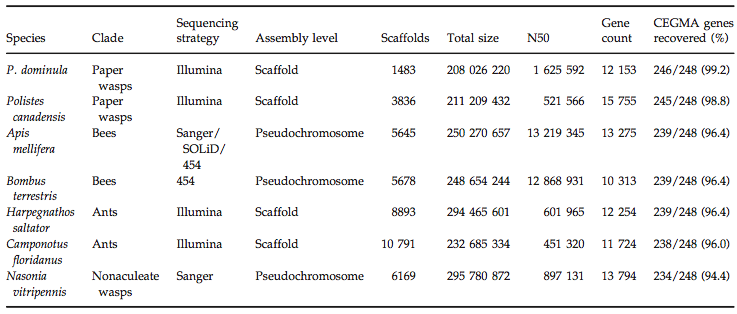
\includegraphics[width=6in]{Assets/Graphics/Pdom/table-01}
%\scriptsize
%\begin{tabularx}{\textwidth}{p{1.75cm}p{1cm}p{1.5cm}p{1.5cm}p{1cm}p{1.5cm}p{1.5cm}p{1cm}p{1.5cm}}
%\hline
%Species                                   &  Clade               &  Sequencing Strategy    &  Assembly Level    &  Scaffolds  &  Total Size   &  N50         &  Gene Count  &  CEGMA Genes Recovered   \\ \hline
%\textit{Polistes     \mbox{dominula}}     &  paper wasps         &  Illumina               &  Scaffold          &  1,483      &  208,026,220  &  1,625,592   &  12,153      &  246/248 (99.2\%)         \\
%\textit{Polistes     \mbox{canadensis}}   &  paper wasps         &  Illumina               &  Scaffold          &  3,836      &  211,209,432  &  521,566     &  15,755      &  245/248 (98.8\%)         \\
%\textit{Apis         \mbox{mellifera}}    &  bees                &  Sanger / SOLiD / 454   &  Pseudo-chromosome &  5,645      &  250,270,657  &  13,219,345  &  13,275      &  239/248 (96.4\%)         \\
%\textit{Bombus       \mbox{terrestris}}   &  bees                &  454                    &  Pseudo-chromosome &  5,678      &  248,654,244  &  12,868,931  &  10,313      &  239/248 (96.4\%)         \\
%\textit{Harpegnathos \mbox{saltator}}     &  ants                &  Illumina               &  Scaffold          &  8,893      &  294,465,601  &  601,965     &  12,254      &  239/248 (96.4\%)         \\
%\textit{Camponotus   \mbox{floridanus}}   &  ants                &  Illumina               &  Scaffold          &  10,791     &  232,685,334  &  451,320     &  11,724      &  238/248 (96.0\%)         \\
%\textit{Nasonia      \mbox{vitripennis}}  &  non-aculeate wasps  &  Sanger                 &  Pseudo-chromosome &  6,169      &  295,780,872  &  897,131     &  13,794      &  234/248 (94.4\%)         \\ \hline
%\end{tabularx}
\label{Table:Pdom1}
\end{table}

The genome assembly appears to be quite complete, on par with other
Illumina-based draft insect genomes
(\protect\hyperlink{ux5fENREFux5f5}{Bonasio \textit{et al.} 2010};
\protect\hyperlink{ux5fENREFux5f37}{Nygaard \textit{et al.} 2011}). CEGMA
analysis (\protect\hyperlink{ux5fENREFux5f42}{Parra \textit{et al.} 2007})
showed 246 (99.2\%) of 248 ultra-conserved core eukaryote genes to be
present in the genome assembly. The total assembled length of the genome
approaches both \textit{in silico} estimates of the \textit{P. dominula}
genome size based on \textit{k}-mer distributions in the sequence data
(246 Mb, see \textbf{SI Results}) and earlier estimates based on flow
cytometry (300 Mb, (\protect\hyperlink{ux5fENREFux5f23}{Johnston
\textit{et al.} 2004})). The gene space of the \textit{P. dominula} genome
therefore appears to be almost completely represented in the assembly,
suggesting that the unrepresented portions of the genome are likely
highly repetitive regions that are difficult to assemble with Illumina
technology.

Automated annotation of \textit{P. dominula} genes was based on a
specifically trained MAKER workflow
(\protect\hyperlink{ux5fENREFux5f6}{Campbell \textit{et al.} 2014}) and
incorporated protein evidence from \textit{Apis mellifera} (NCBI release
102 and OGS 3.2) and \textit{Drosophila} \textit{melanogaster} (FlyBase
r5.55) and transcript data from \textit{P. dominula} (described below),
\textit{P. metricus} (\protect\hyperlink{ux5fENREFux5f2}{Berens \textit{et
al.} 2015a}), and \textit{P. canadensis}
(\protect\hyperlink{ux5fENREFux5f10}{Ferreira \textit{et al.} 2013}). Also
integrated into the annotation were 180 gene models that, during
preliminary stages of annotation, were manually curated and refined
using the yrGATE portal (\protect\hyperlink{ux5fENREFux5f73}{Wilkerson
\textit{et al.} 2006}). This resulted in 11,819 predicted gene models,
designated as release 1.2 (see \textbf{DATA ACCESIBILITY}). Similarity
searches using BLAST revealed most of these predicted genes---10,755 out
of 11,819 (91\%)---have hits to the NCBI non-redundant database, whereas
1,064 show no significant similarity to known proteins. Of the genes
with predicted homologs, most (10,504, or 98\%) have best hits to other
Hymenoptera annotated proteins (\textbf{Figure S3}). These gene models
represent the first whole-genome annotation of a vespid wasp, and
include thousands of high-quality conserved genes enabling more detailed
comparative analysis of hymenopteran genomes, as well as many
species-specific gene models with which to investigate for evidence of
novel clade-specific genes.

\subsection{Composition of \textit{P. dominula} genome shows a combination of
typical hymenopteran as well as unique features.} Comparisons of the
\textit{P. dominula} genome assembly to those of other Hymenoptera
revealed the assembled genome size and proportion of the genome occupied
by transposable elements to be within the range of the other species.
Published hymenopteran genomes show variety in the types and amounts of
transposable element (TE) and other repetitive content, with \textit{Apis
mellifera} harboring almost exclusively a small number of \textit{mariner}
class transposons, and \textit{Nasonia vitripennis} on the other hand
harboring diverse repetitive elements constituting approximately a
quarter of its genome (\protect\hyperlink{ux5fENREFux5f20}{Honeybee
Genome Sequencing Consortium 2006};
\protect\hyperlink{ux5fENREFux5f70}{Werren \textit{et al.} 2010}). The
\textit{Polistes dominula} and \textit{P. canadensis} genomes contain a
fairly low level of repetitive DNA; 11-14\% of the genome assemblies
(24-30 Mb) are estimated to be repetitive, the majority of which
represents simple repeats and low complexity sequence. The two
\textit{Polistes} genomes harbor a very similar cohort of TEs, dominated
in both genomes primarily by L2/CR1/Rex and R1/LOA/Jockey LINEs,
Gypsy/DIRS1 LTRs, and Tc1-IS630-Pogo DNA elements (\textbf{Table S4}).

Characteristics of genome structure were further investigated by parsing
the \textit{P. dominula} genome into 17,888 \textit{interval loci} (iLoci),
each iLocus capturing the local genomic context of a single gene (11,713
iLoci), a cluster of overlapping genes (205 iLoci), or an intergenic
region (5,970 iLoci; see \textbf{SI Methods}). In order to compare a set
of comparable genes across species and rule out differences due to
annotation artifacts, homologous iLoci were determined by computing
iLoci for several additional insect species and clustering their protein
products. A comprehensive comparison included 17 hymenopteran species in
total, but for illustrative purposes, seven representative species
(\textit{P. dominula}, \textit{P. canadensis}, two bees, two ants, and a
non-aculelate, non-social hymenopteran outgroup to the social insects,
\textit{Nasonia vitripennis}) are shown for comparison in this and
subsequent analyses; see \textbf{SI Methods}.

At 11,918, the number of protein-coding iLoci (genes or gene clusters)
in the \textit{P. dominula} genome is well within the range observed in
other Hymenoptera (see \textbf{Figure S5}). However, gene iLoci occupy
only 73.0 Mb (35.1\%) of the \textit{P. dominula} genome (and a similar
proportion was found in \textit{P. canadensis}); this is much less
compared to other species of Hymenoptera in which genes occupy between
140-160 Mb (and 50-65\%) of the assembled genome (\textbf{Figure \ref{Fig:Pdom1}B}).
This difference is due primarily to the annotation of fewer long genes,
and in particular, long introns: while other Hymenoptera have 600-700
gene iLoci 50 kb in length or greater, \textit{P. dominula} has only 84
(see \textbf{Figure \ref{Fig:Pdom1}B}). Further comparative genomic analyses can help
resolve whether this observed reduction in long introns in the \textit{P.
dominula} genome is a truly unique characteristic of the genome
sequence, or whether it stems from differences in annotation workflows.

The \textit{Polistes dominula} genome is also characterized by an
extremely biased nucleotide composition (\textbf{Figure \ref{Fig:Pdom1}C}). With a
genome-wide GC content of 30.8\%, the \textit{P. dominula} genome is the
most biased genome yet reported in Hymenoptera
(\protect\hyperlink{ux5fENREFux5f5}{Bonasio \textit{et al.} 2010};
\protect\hyperlink{ux5fENREFux5f37}{Nygaard \textit{et al.} 2011};
\protect\hyperlink{ux5fENREFux5f54}{Smith \textit{et al.} 2011a};
\protect\hyperlink{ux5fENREFux5f55}{Smith \textit{et al.} 2011b};
\protect\hyperlink{ux5fENREFux5f57}{Suen \textit{et al.} 2011};
\protect\hyperlink{ux5fENREFux5f69}{Weinstock \textit{et al.} 2006};
\protect\hyperlink{ux5fENREFux5f70}{Werren \textit{et al.} 2010}) and one
of the most biased known in any animal
(\url{http://www.ncbi.nlm.nih.gov/genome/browse/}). At the resolution of
individual gene loci, however, \textit{P. dominula} is not as GC-poor as
\textit{Apis mellifera} (29.0\% and 24.7\% median GC content,
respectively), the primary factor being the extreme bias of introns in
\textit{A. mellifera} (21.3\% median GC content for \textit{P. dominula}
versus 17.3\% median GC content for \textit{A. mellifera}; the
distribution of intron length is nearly identical for \textit{P. dominula}
and \textit{A. mellifera}). The composition of the \textit{P. canadensis}
genome is slightly less biased than \textit{P. dominula} at all levels of
resolution, but all trends in comparison to \textit{A. mellifera} are
consistent (see \textbf{SI Results}). The biased composition of
\textit{Polistes} genomes raises some compelling questions about the
evolution of genome composition and potential contributing factors such
as bias in DNA mismatch repair and other genome maintenance mechanisms,
as well as the possibility of historically high levels of CpG
methylation and cytosine deamination.

\subsection{Caste-related transcriptome reveals differentially expressed
conserved and novel genes.} Distinct queen and worker castes arise from
the same genome, a phenomenon known as caste polyphenism that is
characteristic of many social insects
(\protect\hyperlink{ux5fENREFux5f56}{Smith \textit{et al.} 2008}).
Differences in gene expression and alternative splicing between castes
has been a topic of intense research interest because it provides a
striking example of environmentally-induced phenotypic plasticity.
Caste-differential expression has been widely investigated in advanced
eusocial honey bees (\protect\hyperlink{ux5fENREFux5f8}{Chen \textit{et
al.} 2012}; \protect\hyperlink{ux5fENREFux5f16}{Grozinger \textit{et al.}
2007}; \protect\hyperlink{ux5fENREFux5f72}{Whitfield \textit{et al.}
2003}) and ants (\protect\hyperlink{ux5fENREFux5f39}{Ometto \textit{et
al.} 2011}; \protect\hyperlink{ux5fENREFux5f52}{Simola \textit{et al.}
2013a}). More recently, high-throughput RNA sequencing technology
(RNA-Seq) has been applied to profile expression in species representing
a wider array of insect sociality, including an incipiently social small
carpenter bee, an intermediately social bumble bee
(\protect\hyperlink{ux5fENREFux5f18}{Harrison \textit{et al.} 2015}) and
two primitively eusocial species of \textit{Polistes} wasps
(\protect\hyperlink{ux5fENREFux5f3}{Berens \textit{et al.} 2015b};
\protect\hyperlink{ux5fENREFux5f10}{Ferreira \textit{et al.} 2013}). New
RNA-Seq data described in this study represent transcriptome data for a
third \textit{Polistes} species, facilitating the discovery not only of
caste-differentially expressed genes in \textit{P. dominula}, but also of
conserved \textit{Polistes}-specific genes.

We performed two lanes of Illumina paired-end RNA-Seq on mRNA isolated
from heads of individual adult workers and active egg-laying queens (six
replicates per group, from the same population as the male used for
genomic DNA sequencing). The RNA-Seq reads were then mapped to 17,888
iLoci using Bowtie (\protect\hyperlink{ux5fENREFux5f29}{Langmead
\textit{et al.} 2009}), with most libraries mapping at an efficiency of
80\%, after which iLocus abundances were estimated using RSEM
(\protect\hyperlink{ux5fENREFux5f31}{Li \& Dewey 2011}) and tested for
differential expression using EBSeq
(\protect\hyperlink{ux5fENREFux5f30}{Leng \textit{et al.} 2013}) (methods
and quality control described in detail in \textbf{SI Methods}). We
identified 381 iLoci differentially expressed between queens and workers
(\textbf{Figure \ref{Fig:Pdom2}A}), 100 lacking annotated gene models, 276 containing
a single annotated gene, and 5 containing multiple genes. The majority
of the 381 differentially expressed iLoci (231; 60\%) are up-regulated
in workers. Other reports that also focused on head or brain gene
expression from \textit{Polistes}
(\protect\hyperlink{ux5fENREFux5f3}{Berens \textit{et al.} 2015b};
\protect\hyperlink{ux5fENREFux5f10}{Ferreira \textit{et al.} 2013}) and
honey bees (\protect\hyperlink{ux5fENREFux5f16}{Grozinger \textit{et al.}
2007}) also found the majority of genes are worker-biased in expression.
The skew towards worker-biased expression could reflect differences in
behavioral flexibility and/or cognitive demands of workers compared to
egg-laying queens (\protect\hyperlink{ux5fENREFux5f38}{O'Donnell
\textit{et al.} 2011}).

Differentially expressed iLoci are significantly enriched for Gene
Ontology functions in fatty acid metabolism, neurotransmitter activity,
and amino acid metabolism when compared to the background set of all
\textit{P. dominula} gene models (\textbf{Figure \ref{Fig:Pdom2}B}). Previous studies on
caste-related gene expression in other \textit{Polistes} species have also
identified consistent differences in the expression of genes related to
lipid metabolism (\protect\hyperlink{ux5fENREFux5f3}{Berens \textit{et
al.} 2015b}; \protect\hyperlink{ux5fENREFux5f59}{Sumner \textit{et al.}
2006}; \protect\hyperlink{ux5fENREFux5f62}{Toth \textit{et al.} 2010}).
These data contribute to a growing base of information suggesting the
expression of deeply conserved genes (i.e. a ``genetic toolkit'')
related to metabolism is related to caste differences and may play a key
role in the evolution of caste-containing insect societies
(\protect\hyperlink{ux5fENREFux5f61}{Toth \& Robinson 2007}).

All previously examined insects show evidence of large amounts of
alternative splicing, including other social insect genomes
(\protect\hyperlink{ux5fENREFux5f11}{Flores \textit{et al.} 2012};
\protect\hyperlink{ux5fENREFux5f32}{Li-Byarlay \textit{et al.} 2013}). As
expected, we found evidence for alternative splicing in 1,743 of the
\textit{P. dominula} gene models. In particular, \textit{via} transcript
mapping and scanning for the two major types of alternative splicing
(intron retention and exon skipping, see \textbf{SI Methods}) we
uncovered 1,616 intron retention events in 1,135 genes and 1,720 exon
skipping events in 884 genes (see \textbf{SI Results}). 859 genes show
only intron retention, 608 genes show only exon skipping, and 276 genes
show both. However, analysis with Cufflinks and Cuffdiff \{Trapnell,
2013 \#520\}(\protect\hyperlink{ux5fENREFux5f64}{Trapnell \textit{et al.}
2013}) reported no cases of caste differential splicing, suggesting
alternative splicing is not related to adult caste differences, at least
in heads, of \textit{P. dominula.}

Recently, there has been growing interest in the potential for
``novel'', or taxonomically restricted genes in the evolution of novel
phenotypes and in particular, eusociality
(\protect\hyperlink{ux5fENREFux5f58}{Sumner 2014}). We also used our
transcriptome data, in conjunction with previously published data for
other \textit{Polistes} species, to search for well-supported
\textit{Polistes-}specific genes. Our data represent the third published
transcriptome dataset for a \textit{Polistes} species, together with the
transcriptomes of two New World species, \textit{Polistes metricus}
(\protect\hyperlink{ux5fENREFux5f3}{Berens \textit{et al.} 2015b}) and the
Neotropical \textit{Polistes canadensis}
(\protect\hyperlink{ux5fENREFux5f10}{Ferreira \textit{et al.} 2013}). In
the \textit{Polistes canadensis} study, the authors identified a large
number of novel transcripts (approximately 50\% of sequenced
transcripts) with no similarity to any known sequence and suggest that
novel genes may be related to the evolution of caste differences in
social insects (\protect\hyperlink{ux5fENREFux5f58}{Sumner 2014}). We
performed a more in-depth exploration of the three transcriptomes in
order to identify \textit{Polistes}-specific transcripts that were shared
by all three species. Such transcripts are much more likely to represent
true protein-coding genes because they are conserved across species and
there is evidence of their expression in multiple species. Considering
\textit{P. dominula} transcripts with an open reading frame of at least 80
aa, we found 19,173 transcripts with no significant similarity to
Hexapoda sequences. Only 144 of these transcripts have translation
products that are conserved between all three \textit{Polistes}
transcriptomes. Of the 144 conserved shared transcripts, 118 are found
in the annotated genome assembly, aligning to 93 different iLoci
(\textbf{Figure \ref{Fig:Pdom2}C}). Only 10 of these 93 iLoci also have evidence of
\textit{Polistes}-specific genes from the genome annotation (in the form
of gene models without matches to protein databases), and even in these
10 cases there is little agreement between transcript alignment
structure and predicted gene structure (\textbf{Table S11}). These
results suggest that while single lines of evidence may offer hints of
clade-specific genes, very few cases are well supported when subjected
to multiple lines of inquiry. This confirms a recent study in ants that
uncovered evidence for very few shared, genus-specific genes and more
unique species-specific gene, some of which are likely bioinformatics
artifacts (\protect\hyperlink{ux5fENREFux5f52}{Simola \textit{et al.}
2013a}).

There are conflicting reports on the association of novel transcripts in
caste differences in \textit{Polistes}. Transcriptomic comparisons from
\textit{P. canadensis} adults suggested novel transcripts are more likely
to be caste-biased in expression
(\protect\hyperlink{ux5fENREFux5f10}{Ferreira \textit{et al.} 2013}),
whereas novel transcripts from \textit{P. metricus} larvae did not show
this caste-bias (\protect\hyperlink{ux5fENREFux5f3}{Berens \textit{et al.}
2015b}). In the current study, we found that 77 out of 93 iLoci (83\%)
associated with the 144 well-supported \textit{Polistes-}specific
transcripts are caste differentially expressed (significantly
overrepresented, Fisher's Exact Test p \textless{} 2.2e-16), 34 of which
(44\%) are up-regulated in workers. In addition, eight of the 10 iLoci
containing both unmatched transcripts and unmatched gene models are
caste differentially expressed, with 4/8 up-regulated in workers. These
results are consistent with data from \textit{P. canadensis}
(\protect\hyperlink{ux5fENREFux5f10}{Ferreira \textit{et al.} 2013})
suggesting novel genes are more likely to be caste-biased in expression
in adults. The fact that a similar relationship between caste-biased
expression and novel genes was not found in \textit{P. metricus} larvae
suggests there could be different functions for novel genes across
species and/or life stages.

\subsection{DNA methylation system is greatly reduced in \textit{P.
dominula}.} There has been great interest in the role of epigenetics in
eusociality, and data from honey bees has generated considerable
interest in the potential role of DNA methylation in the regulation of
gene expression during the development of queen and worker castes
(\protect\hyperlink{ux5fENREFux5f34}{Lyko \& Maleszka 2011}). We used
the aforementioned genome and transcriptome data from \textit{P.
dominula}, along with newly generated whole genome bisulfite sequencing
(methylome) data, to probe the presence and extent of caste-association
of DNA methylation in the independently evolved social paper wasps.

A full complement of DNA methyltransferases, \textit{Dnmt1, 2,} and
\textit{3,} is considered to be necessary for a fully functional DNA
methylation system (\protect\hyperlink{ux5fENREFux5f34}{Lyko \& Maleszka
2011}). \textit{Dnmt1} is typically considered as the ``maintenance''
methyltransferase involved in maintaining consistent methylation across
cell divisions and generations (\protect\hyperlink{ux5fENREFux5f34}{Lyko
\& Maleszka 2011}). \textit{Dnmt2} is thought to be involved mainly in the
methylation of transfer RNAs. \textit{Dnmt3} is the ``de novo''
methyltransferase, and has been suggested to be related more to
environmentally-responsive DNA methylation that occurs within the
lifetime of an individual (\protect\hyperlink{ux5fENREFux5f34}{Lyko \&
Maleszka 2011}). Other canonical methylation-related proteins include
MBD (Methyl-CpG-binding domain protein) and the demethylation enzyme TET
(Ten-eleven translocation methylcytosine dioxygenase)
(\protect\hyperlink{ux5fENREFux5f34}{Lyko \& Maleszka 2011}). We used
BLAST to identify sets of homologs for each of these genes and subjected
these sets of sequences to molecular phylogeny analysis to determine
copy numbers of each of these five major DNA methylation related genes.

All previously sequenced Hymenoptera possess a full complement of DNA
methyltransferases (\protect\hyperlink{ux5fENREFux5f75}{Yan \textit{et
al.} 2015}), except the recently sequenced \textit{Polistes canadensis}
which lacks \textit{Dnmt3} (\protect\hyperlink{ux5fENREFux5f43}{Patalano
\textit{et al.} 2015}). Our MAKER annotation workflow (augmented by manual
annotations as well as low stringency similarity searches for
potentially incomplete or highly diverged homologs) also uncovered no
\textit{Dnmt3} gene, but did identify one \textit{Dnmt1} gene (as in ants
(\protect\hyperlink{ux5fENREFux5f5}{Bonasio \textit{et al.} 2010}), as
opposed to two in honey bees (\protect\hyperlink{ux5fENREFux5f66}{Wang
\textit{et al.} 2006})) and one \textit{Dnmt2} gene, as well as genes
encoding MBD and TET homologs (summarized in \textbf{Figure \ref{Fig:Pdom3}A}). To
further investigate whether the absence of a \textit{Dnmt3} gene model
might represent a gene loss, we examined available Hymenoptera genomes
for shared synteny in the region harboring \textit{Dnmt3} in \textit{Apis
mellifera}. Results show that the \textit{Dnmt3} locus is within a
syntenic block encompassing at least an additional two genes upstream
and two genes downstream, conserved in bee and ant genomes. Synteny
analyses were conducted with the SynFind and associated tools within the
CoGe platform (\url{https://genomevolution.org/coge/};
\protect\hyperlink{ux5fENREFux5f60}{Tang \textit{et al.} (2015)}). Sample
genome alignments are shown in \textbf{Figure \ref{Fig:Pdom3}B}. The first upstream
and the two downstream genes co-localize in a 90kb region on
scaffold0086 of our \textit{P. dominula} assembly, preserving the syntenic
block (the leftmost gene of the bee-ant syntenic block is preserved on
scaffold0049 but would be at least 235 kb away if this scaffold were to
align upstream of scaffold0086). However, there is a conspicuous absence
of any similarity to \textit{Dnmt3} in the syntenic region of the \textit{P.
dominula} genome (\textbf{Figure \ref{Fig:Pdom3}B}). Intriguingly, across the
remaining Hymenoptera species, the region upstream of the annotated
\textit{Dnmt3} genes encoding the conserved C-terminus of the
methyltransferase is highly variable in size and gene structure
annotation is unclear (including annotation of the possibly overlapping
upstream gene). The \textit{Nasonia vitripennis} \textit{Dnmt3} protein is
highly diverged at the N-terminus, and although the other genes of the
bee-ant syntenic block are highly conserved in \textit{Nasonia}, they are
widely spread in the genome. These results suggest that the \textit{Dnmt3}
locus, and by extension, perhaps some functional aspects of DNA
methylation systems in general, are not highly conserved in different
lineages of Hymenoptera.

In addition to the lack of genome sequence evidence for a functional
\textit{Dnmt3} gene in \textit{Polistes dominula}, we found no significant
similarity between Hymenoptera \textit{Dnmt3} sequences and transcripts
from any of the three \textit{Polistes} species' transcriptomes
(\protect\hyperlink{ux5fENREFux5f3}{Berens \textit{et al.} 2015b};
\protect\hyperlink{ux5fENREFux5f10}{Ferreira \textit{et al.} 2013})
(tblastn search with -evalue 1e-8). The lack of any \textit{Dnmt3}
transcripts in the three congeners strongly suggests this gene has
indeed been lost across the genus \textit{Polistes.} Further work on
additional species will be necessary to determine whether this loss is
common to the entire paper wasp family Vespidae.

Along with the loss of \textit{Dnmt3,} whole genome bisulfite sequencing
of one pool of queen and one pool of worker heads revealed a dramatic
reduction in DNA methylation in \textit{P. dominula} compared to other
Hymenoptera. This is in contrast to previous reports suggesting the
presence of typical amounts of DNA methylation in \textit{P. dominula},
but these reports used a less reliable method for estimating DNA
methylation based on a methylation-sensitive restriction enzyme assay
(\protect\hyperlink{ux5fENREFux5f26}{Kronforst \textit{et al.} 2008};
\protect\hyperlink{ux5fENREFux5f67}{Weiner \textit{et al.} 2013}). Through
a complete and uniform reanalysis of previously published Hymenoptera
bisulfite sequencing data (from honey bees, two ant species,
\textit{Polistes canadensis,} and \textit{Nasonia vitripennis}) we were able
to make a reliable comparison of DNA methylation levels in \textit{P.
dominula} to those of other Hymenoptera (described in \textbf{SI
Methods}). Overall, levels of DNA methylation in \textit{P. dominula} are
more than two orders of magnitude lower than in other Hymenoptera. This
includes the congeneric \textit{Polistes canadensis}, which, although
showing lower levels of methylation than ants and bees, still has two
orders of magnitude more methylated CpG sites than \textit{P. dominula}
(\textbf{Figure \ref{Fig:Pdom3}C}, \textbf{SI Results})\textit{.} We uncovered only 124
and 158 CpG methylated sites, respectively in the queen and worker
samples; this is in stark contrast to tens of thousands of sites
uncovered in all of the other Hymenoptera species (\textbf{Figure \ref{Fig:Pdom3}C}).
Similar to other insects (\protect\hyperlink{ux5fENREFux5f45}{Rasmussen
\& Amdam 2015}), most methylated sites were found within genes (74 and
89 sites in queen and worker samples, respectively); see \textbf{SI
Results}. Strikingly, methylation was targeted to the same seven genes
in both queen and worker samples (\textbf{Figure \ref{Fig:Pdom3}D}), and several of
these have putative functions related to DNA binding. Thus, there were
zero caste differentially methylated genes, and great similarity between
castes, even at the level of which cytosines within the seven genes were
methylated. Of the 101 total methylated cytosines within the seven
genes, 62 (61\%) of the same methylated cytosines were shared between
both castes (\textbf{Figure \ref{Fig:Pdom3}D}). This result is again in contrast to
studies from both bees (\protect\hyperlink{ux5fENREFux5f33}{Lyko
\textit{et al.} 2010}) and ants
(\protect\hyperlink{ux5fENREFux5f4}{Bonasio \textit{et al.} 2012}), which
reported hundreds of caste differentially methylated genes between queen
and worker castes. The fact that nearly identical methylation patterns
were found in just a few genes, but consistently across castes, suggests
the extremely low level of DNA methylation we describe in \textit{P.
dominula} is real and may be of some functional significance. We suggest
that, despite a massive reduction in \textit{de novo} methylation in paper
wasps, there may have been selection to retain ``maintenance
methylation'', likely \textit{via} the action of of \textit{Dnmt1,} for a
few key genes. This idea is supported by the observation that five out
of the seven \textit{P. dominula} methylated genes also showed strong
methylation in \textit{P. canadensis} (\textbf{SI Results}), and homologs
of three of these seven genes in \textit{Apis mellifera} are methylated
consistently across multiple independently published experiments.

Our methylome data from \textit{P. dominula} also suggest no clear
connection to dynamic gene expression patterns: none of the seven
methylated genes is differentially expressed between castes; two out of
the seven show some evidence of alternative splicing, but not caste
differential splicing (PdomGENEr1.2-09385 and PdomGENEr1.2-09184).
Although \textit{P. canadensis} also shows some evidence of a reduced
methylation system (loss of \textit{Dnmt3} and fewer methylated CpG sites
and methylated genes than bees and ants
(\protect\hyperlink{ux5fENREFux5f43}{Patalano \textit{et al.} 2015})), the
reduction in \textit{P. dominula} is much more striking. This suggests
reduced DNA methylation systems may be a general characteristic of paper
wasps, but that there has been even further reduction of these systems
in the \textit{P. dominula} lineage relative to some of its congeners.

These data raise intriguing questions about the importance and function
of DNA methylation in insects. DNA methylation systems have also been
dramatically reduced in other insect lineages (e.g. \textit{Drosophila}
flies and \textit{Tribolium} beetles), the shared feature being a loss of
\textit{Dnmt3} and large reduction in overall levels of DNA methylation
(\protect\hyperlink{ux5fENREFux5f13}{Glastad \textit{et al.} 2011}).
Furthermore, there are other insects where \textit{Dnmt3} is not present,
but moderate levels of DNA methylation remain
(\protect\hyperlink{ux5fENREFux5f36}{Mita \textit{et al.} 2004};
\protect\hyperlink{ux5fENREFux5f43}{Patalano \textit{et al.}
2015})\textit{.} Thus, DNA methylation is not clearly related to gene
regulation in some insects (\protect\hyperlink{ux5fENREFux5f12}{Glastad
\textit{et al.} 2014}) and even some social insects, suggesting other
types of epigenetic mechanisms such as histone modifications
(\protect\hyperlink{ux5fENREFux5f53}{Simola \textit{et al.} 2013b}) or
microRNAs may be more important. Our data also highlight the surprising
lability of epigenetic mechanisms even within an insect lineage
(Hymenoptera) and do not support the idea that phenotypic plasticity
afforded by DNA methylation is required for the evolution of castes in
social insects (\protect\hyperlink{ux5fENREFux5f68}{Weiner \& Toth
2012}).

We also examined patterns of occurrence of CpG dinucleotides in the
\textit{P. dominula} genome, because segmental ratios of observed to
expected (o/e) CpG frequency have been used as an indicator of regional
DNA methylation status, based on the assumption that highly methylated
regions are characterized by mutational loss of methylated cytosines
(\protect\hyperlink{ux5fENREFux5f76}{Yi \& Goodisman 2009}). The
distribution of CpG o/e in \textit{P. dominula} is similarly broad as that
of other Hymenoptera, but lacking the bimodal distribution
characteristic of the measure in bee coding regions (\textbf{Figure
S8}). Use of this measure as an indicator of methylation status in
\textit{P. dominula} would have incorrectly inferred the presence of
numerous methylated genes. Thus, the CpG o/e measure does not accurately
reflect the true methylation status of the \textit{P. dominula} genome
based on bisulfite sequencing, a much more direct and sensitive method
for detecting actual site-specific methylation. It is conceivable that
CpG depletion is still correlated with historical (not modern) patterns
of DNA methylation, and this is reflected in the fairly typical CpG o/e
distribution in \textit{P. dominula} (\textbf{Figure S8})\textit{.} Because
appreciable levels of DNA methylation are found in a wide variety of
other Hymenoptera (\textbf{Figure \ref{Fig:Pdom3}A}), it is likely that reduced DNA
methylation is a derived condition in \textit{Polistes}, but more data on
additional species are needed to understand when and why reduced DNA
methylation evolved in vespid wasps.

\subsection{Aculeate Phylogeny.} The genome of \textit{Polistes dominula}
provides a beneficial complement to the genomes of several species of
aculeate Hymenoptera already published. Together, these genomes are a
powerful comparative genomics resource for identifying what is conserved
and what is unique among the primary aculeate lineages. A delineation of
the phylogenetic relationships between these lineages is a fundamental
component for analysis and interpretation of evolved traits, and yet
consensus regarding the phylogeny of Aculeata remains elusive
(\protect\hyperlink{ux5fENREFux5f22}{Johnson \textit{et al.} 2013};
\protect\hyperlink{ux5fENREFux5f44}{Pilgrim \textit{et al.} 2008}). A
study using molecular data from 4 loci in 64 taxa placed bees
(superfamily Apoidea) as sister to scoliid and bradynobaenid wasps
(\protect\hyperlink{ux5fENREFux5f44}{Pilgrim \textit{et al.} 2008}), while
a more recent study involving analysis of 308 genes from 19 taxa found
ants (family Formicidae) to be sister to bees
(\protect\hyperlink{ux5fENREFux5f22}{Johnson \textit{et al.} 2013}).

Because our current work describes the one of the first published
complete genomes of a vespid wasp, we sought to use these data to
investigate the phylogenetic grouping of \textit{Polistes} proteins
relative to orthologs in bees, ants, and the non-aculeate wasp
\textit{Nasonia} as an outgroup. Using conserved single-copy orthologs
present in \textit{Apis mellifera} (bee), \textit{Harpegnathos saltator}
(ant), \textit{Polistes dominula} (paper wasp), and \textit{Nasonia
vitripennis} (non-aculeate outgroup), we inferred a phylogenetic tree
for each gene using these four representative protein sequences (see
\textbf{SI Methods}). We observed all possible topologies in the 2,077
gene trees: bees and ants as closest neighbors in 889 trees (43\%),
\textit{Polistes} and bees as closest in 696 trees (34\%), and
\textit{Polistes} and ants as closest in 492 trees (24\%). Although the
most common topology (bees and ants as closest) agrees with the results
of the most recent, transcriptome-based phylogenetic analysis of
aculeates (45), there was definitely not a clear consensus from our
data. Based on our analysis, the protein-coding genomes of the published
Hymenoptera do not yet provide a definitive answer to the question of
the phylogenetic relationship of bees, ants, and vespid wasps.
Additional aculeate genomes, including more representatives of the
Vespidae (\protect\hyperlink{ux5fENREFux5f21}{Jandt \& Toth 2015}) and
other wasp families, may help to better resolve aculeate relationships
in the future.

\section{Conclusions}

This paper provides valuable and comprehensive genomic resources for one
of the major lineages of eusocial insects, the vespid wasps, represented
by the behavioral model species \textit{Polistes dominula}. The \textit{P.
dominula} genome is a relatively compact (250Mb) genome with little
repetitive DNA, as well as low GC content, in comparison to other
Hymenoptera. Transcriptomic analyses revealed several hundred genes with
caste-related expression, with functions related to fatty acid and amino
acid metabolism and neurotransmitter activity. In addition, we
identified several \textit{Polistes-}specific genes, several of which also
show differential expression between queen and worker castes. Together,
these data provide some support for the roles of both conserved genes
and novel genes in the evolution and maintenance of caste differences in
social wasps (\protect\hyperlink{ux5fENREFux5f58}{Sumner 2014};
\protect\hyperlink{ux5fENREFux5f61}{Toth \& Robinson 2007}). The most
surprising finding from our \textit{P. dominula} --omics data was clear
evidence of a striking reduction in the DNA methylation system. \textit{P.
dominula} have a reduced complement of DNA methylation enzymes,
including a loss of the \textit{de novo} methyltransferase \textit{Dnmt3},
as well as extremely reduced levels of DNA methylation in the
genome---with evidence for just over 100 methylated sites in only seven
genes. In addition, there was no relationship between DNA methylation
and caste- related gene expression, methylation, nor alternative
splicing. There has been great interest and research activity related to
the potential role of DNA methylation in the regulation of caste
differences and caste evolution in eusocial insects
(\protect\hyperlink{ux5fENREFux5f28}{Kucharski \textit{et al.} 2008};
\protect\hyperlink{ux5fENREFux5f68}{Weiner \& Toth 2012}). Our data are
novel in that they suggest \textit{P. dominula} possesses the most reduced
DNA methylation system known for any eusocial insect, but there are
other examples of non-social insects with similarly reduced methylation
systems, including \textit{Drosophila}. These data add to growing evidence
for a surprising amount of lability of epigenetic mechanisms in insects,
and suggest DNA methylation \textit{per se} is not generally related to
the evolution of castes in social insects. These genomic,
transcriptomic, and epigenomic data on a primitively eusocial vespid
wasp open up exciting new possibilities for comparative genomics of
social evolution. Comparisons both across eusocial lineages and within
lineages have the potential to provide new insights into the roles of
conserved genes and pathways, novel genes, and epigenetic mechanisms in
social evolution (\protect\hyperlink{ux5fENREFux5f47}{Rehan \& Toth
2015}).

\section{Acknowledgments}

This work was supported in part by the U.S.A. National Science
Foundation grant NSF-IOS-1311512 and a grant from the Iowa State
University Center for Integrated Animal Genomics, both awarded to AT. DS
was supported in part by NSF award \#1221984 to VB.

The authors would like to thank Amy Geffre for assistance with DNA and
RNA extractions, Susan Weiner for preliminary work on DNA
methyltransferase genes, and members of the Toth lab for reviewing the
manuscript. We also thank Michael Goodisman and Brendan Hunt for
discussions about methylome sequencing and DNA methylation patterns. We
also thank Christina Grozinger, Stefano Turillazzi, Gene Robinson, and
Joan Strassmann for helpful discussions and support in planning stages
of this project, and GR and JS for comments on the manuscript. We also
thank our manual annotation team: Arian Avalos, Seth Barribeau,
Katherine Noble, Sandra Rehan, Fabio Manfredini, Griffin Smith, Amy
Geffre, Adam Dolezal, Jimena Carrillo-Tripp, Alexander Walton, and
Jennifer Jandt for submitting manual gene annotations; and Jon Duvick
for reviewing and curating annotation submissions.

\section{Data Accessibility}

Raw Illumina sequences are available from the NCBI Short Read Archive
under the following accessions: accession SAMN02584905 for whole genome
shotgun reads; accessions SAMN03940809-SAMN03940820 for RNA sequence
reads; and accessions SAMN03946123 and SAMN03946134 for bisulfite
sequence reads. The genome assembly is available from GenBank under the
accession GCA\_001465965.1, and the transcriptome shotgun assembly is
available from GenBank under the accession GEDB00000000.1.

Additional supporting data, analysis documentation, and supporting code
have been deposited in the fig\textbf{share} archive and in several
GitHub repositories, as described at
\url{https://pdomgenomeproject.github.io/}.

Sequences, annotations, and alignments are also available through
PdomGDB, an integrated data resource including a genome browser, a BLAST
server, and a community annotation portal (see
\url{http://goblinx.soic.indiana.edu/PdomGDB}).

\section{Author Contributions}

All computational analyses of the data were done by DS and VB at Indiana
University.~ AB assisted with the assembly of the \textit{P. dominula}
transcriptome and with differential expression analysis.~~AS contributed
to preliminary identification of transposable and repetitive elements,
and to analysis of telomere-related genes and sequence motifs.~~KG
contributed template Perl code for preliminary analyses of CpG o/e.~ AT
conceived of and oversaw the project, interpreted results, and collected
and processed wasp samples.~ DS, VB, and AT wrote the manuscript.

\section{Figures}

\subsection*{Figure \ref{Fig:Pdom1}}
\noindent
\textbf{A}. Best supported molecular phylogeny of the eusocial aculeate Hymenoptera based on recent transcriptome studies and analysis of 2,077 conserved genes reported in this study.
\textbf{B}. Stacked bar plot showing genome content of \textit{Polistes dominula} broken down by the proportion occupied by various categories of gene content and conservation, compared to another paper wasp (green labels), two bees (black labels), two ants (red labels), and the outgroup \textit{Nasonia vitripennis}. See also \textbf{Figure S5}.
\textbf{C}. Stacked rug plot showing nucleotide composition of long genomic sequences from 3 bees (in black), 2 ants (in red), the outgroup
\textit{Nasonia vitripennis} (in blue), and 2 paper wasps (in green). Each vertical bar represents a chromosome, linkage group, or scaffold at least 1 Mb in length.
Photo credits: \textit{N. vitripennis} by E. Cash and J. Gibson;
\textit{P. dominula} by S. McCann; \textit{S. invicta} and \textit{A. mellifera} by A. Wild.

\subsection*{Figure \ref{Fig:Pdom2}}
\noindent
\textbf{A}. Heatmap of expression values of 367 differentially expressed interval loci (iLoci). The blue color indicates overexpression, while the yellow indicates underexpression. 212 iLoci (58\%) of the differentially expressed iLoci are overexpressed in workers.
\textbf{B}. Bar chart showing the representation of eight GO functional categories as a proportion of differentially expressed iLoci (blue bars) versus all iLoci (red bars), determined by an enrichment analysis to be overrepresented in differentially expressed iLoci.
\textbf{C}. Putative \textit{Polistes-}specific genes, defined as unmatched transcripts with significant pairwise protein-level similarity among three Polistes species (Pd for \textit{P. dominula}, Pc for \textit{P. canadensis}, and Pm for \textit{P. metricus}). Because of variation in gene copy number and number of alternative transcript isoforms, the number of transcripts in each intersection of the diagram is different for each species, and only the smallest number is shown. For example, the 3-species intersection consists of 144 transcripts from \textit{P. dominula}, 136 transcripts from \textit{P. canadensis}, and 95 transcripts from \textit{P. metricus}.

\subsection*{Figure \ref{Fig:Pdom3}}
\noindent
\textbf{A}. Copy number of five methylation-related genes in the primary Hymenoptera lineages.
\textbf{B}. Evidence for shared synteny around the \textit{Dnmt3} locus in bee, paper wasp, and ant genomes. Colored bars represent conserved coding regions between \textit{Polistes dominula} (top track) and \textit{Apis mellifera} (black blocks), \textit{Bombus terrestris} (grey blocks), and \textit{Camponotus floridanus} (red blocks). Regions of similarity are largely collinear (shown for the \textit{Apis mellifera} to \textit{Camponotus floridanus} comparison by the blue lines connecting the similar blocks). Gene models are shown by arrow structures with coding exons in green, UTRs in blue, and introns as thin lines. Each gene is denoted by a numbered box as follows: 1) GenBank protein entries XP\_006568814 (26S proteasome non-ATP regulatory subunit 6-like), 2) XP\_006568813 (uncharacterized), XP\_00658716 (Dnmt3), 4) XP\_006568806 (polynucleotide 5'-hydroxyl-kinase NOL9-like), and 5) XP\_0065688112 (histone lysine demethylase PHF8-like) in \textit{A. mellifera} (linkage group LG2, GenBank NC\_007071), from left to right. The lack of similarity blocks around 50K on the \textit{P. dominula} scale demonstrates the postulated loss of \textit{Dnmt3} in this species.
\textbf{C}. Bar chart showing the number of CpGs with a high level of support for methylation from bisulfite sequence data. The number of highly supported methylation sites for each species is based on pooled reads for all available samples, and is shown for one bee (black), two ants (red, note that ``worker'' refers to ``minor workers'' in \textit{C. floridanus}), two paper wasps (green), and \textit{N. vitripennis} (blue).
\textbf{D.} Gene models for the 7 \textit{P. dominula} methylated genes (with corresponding Gene ID numbers and putative annotations based on best BLAST hits). Approximate locations of each of the 124 highly supported methylation sites within each gene are indicated with a line-dot symbol, with sites methylated in both queen and worker samples (n=76) indicated in black, sites methylated in just the queen sample in green (n=18), and sites methylated in just the worker sample (n=30) in orange.

\begin{figure}[h]
\centering
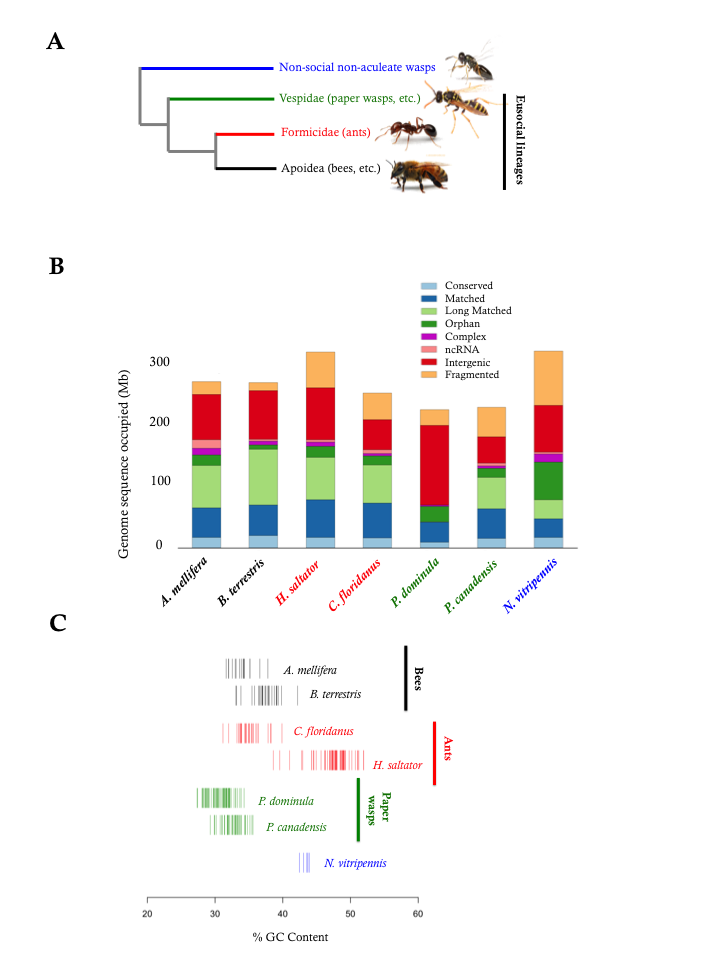
\includegraphics[width=6in]{Assets/Graphics/Pdom/figure-1}
\caption{~}
\label{Fig:Pdom1}
\end{figure}

\begin{figure}[h]
\centering
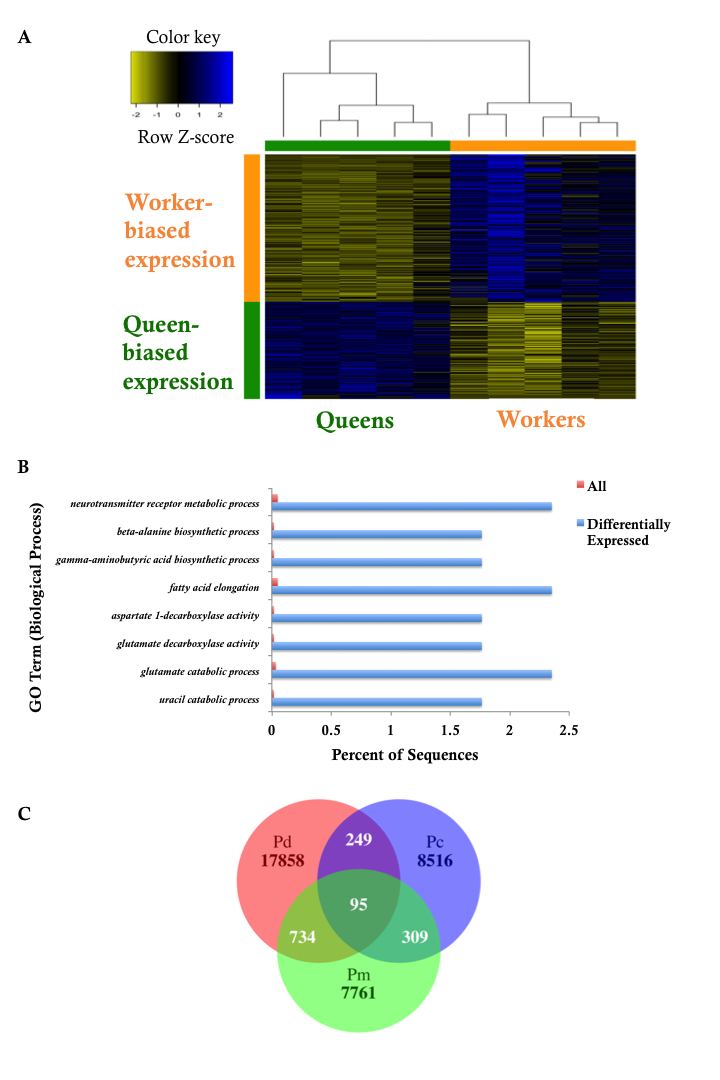
\includegraphics[width=6in]{Assets/Graphics/Pdom/figure-2}
\caption{~}
\label{Fig:Pdom2}
\end{figure}

\begin{sidewaysfigure}[h]
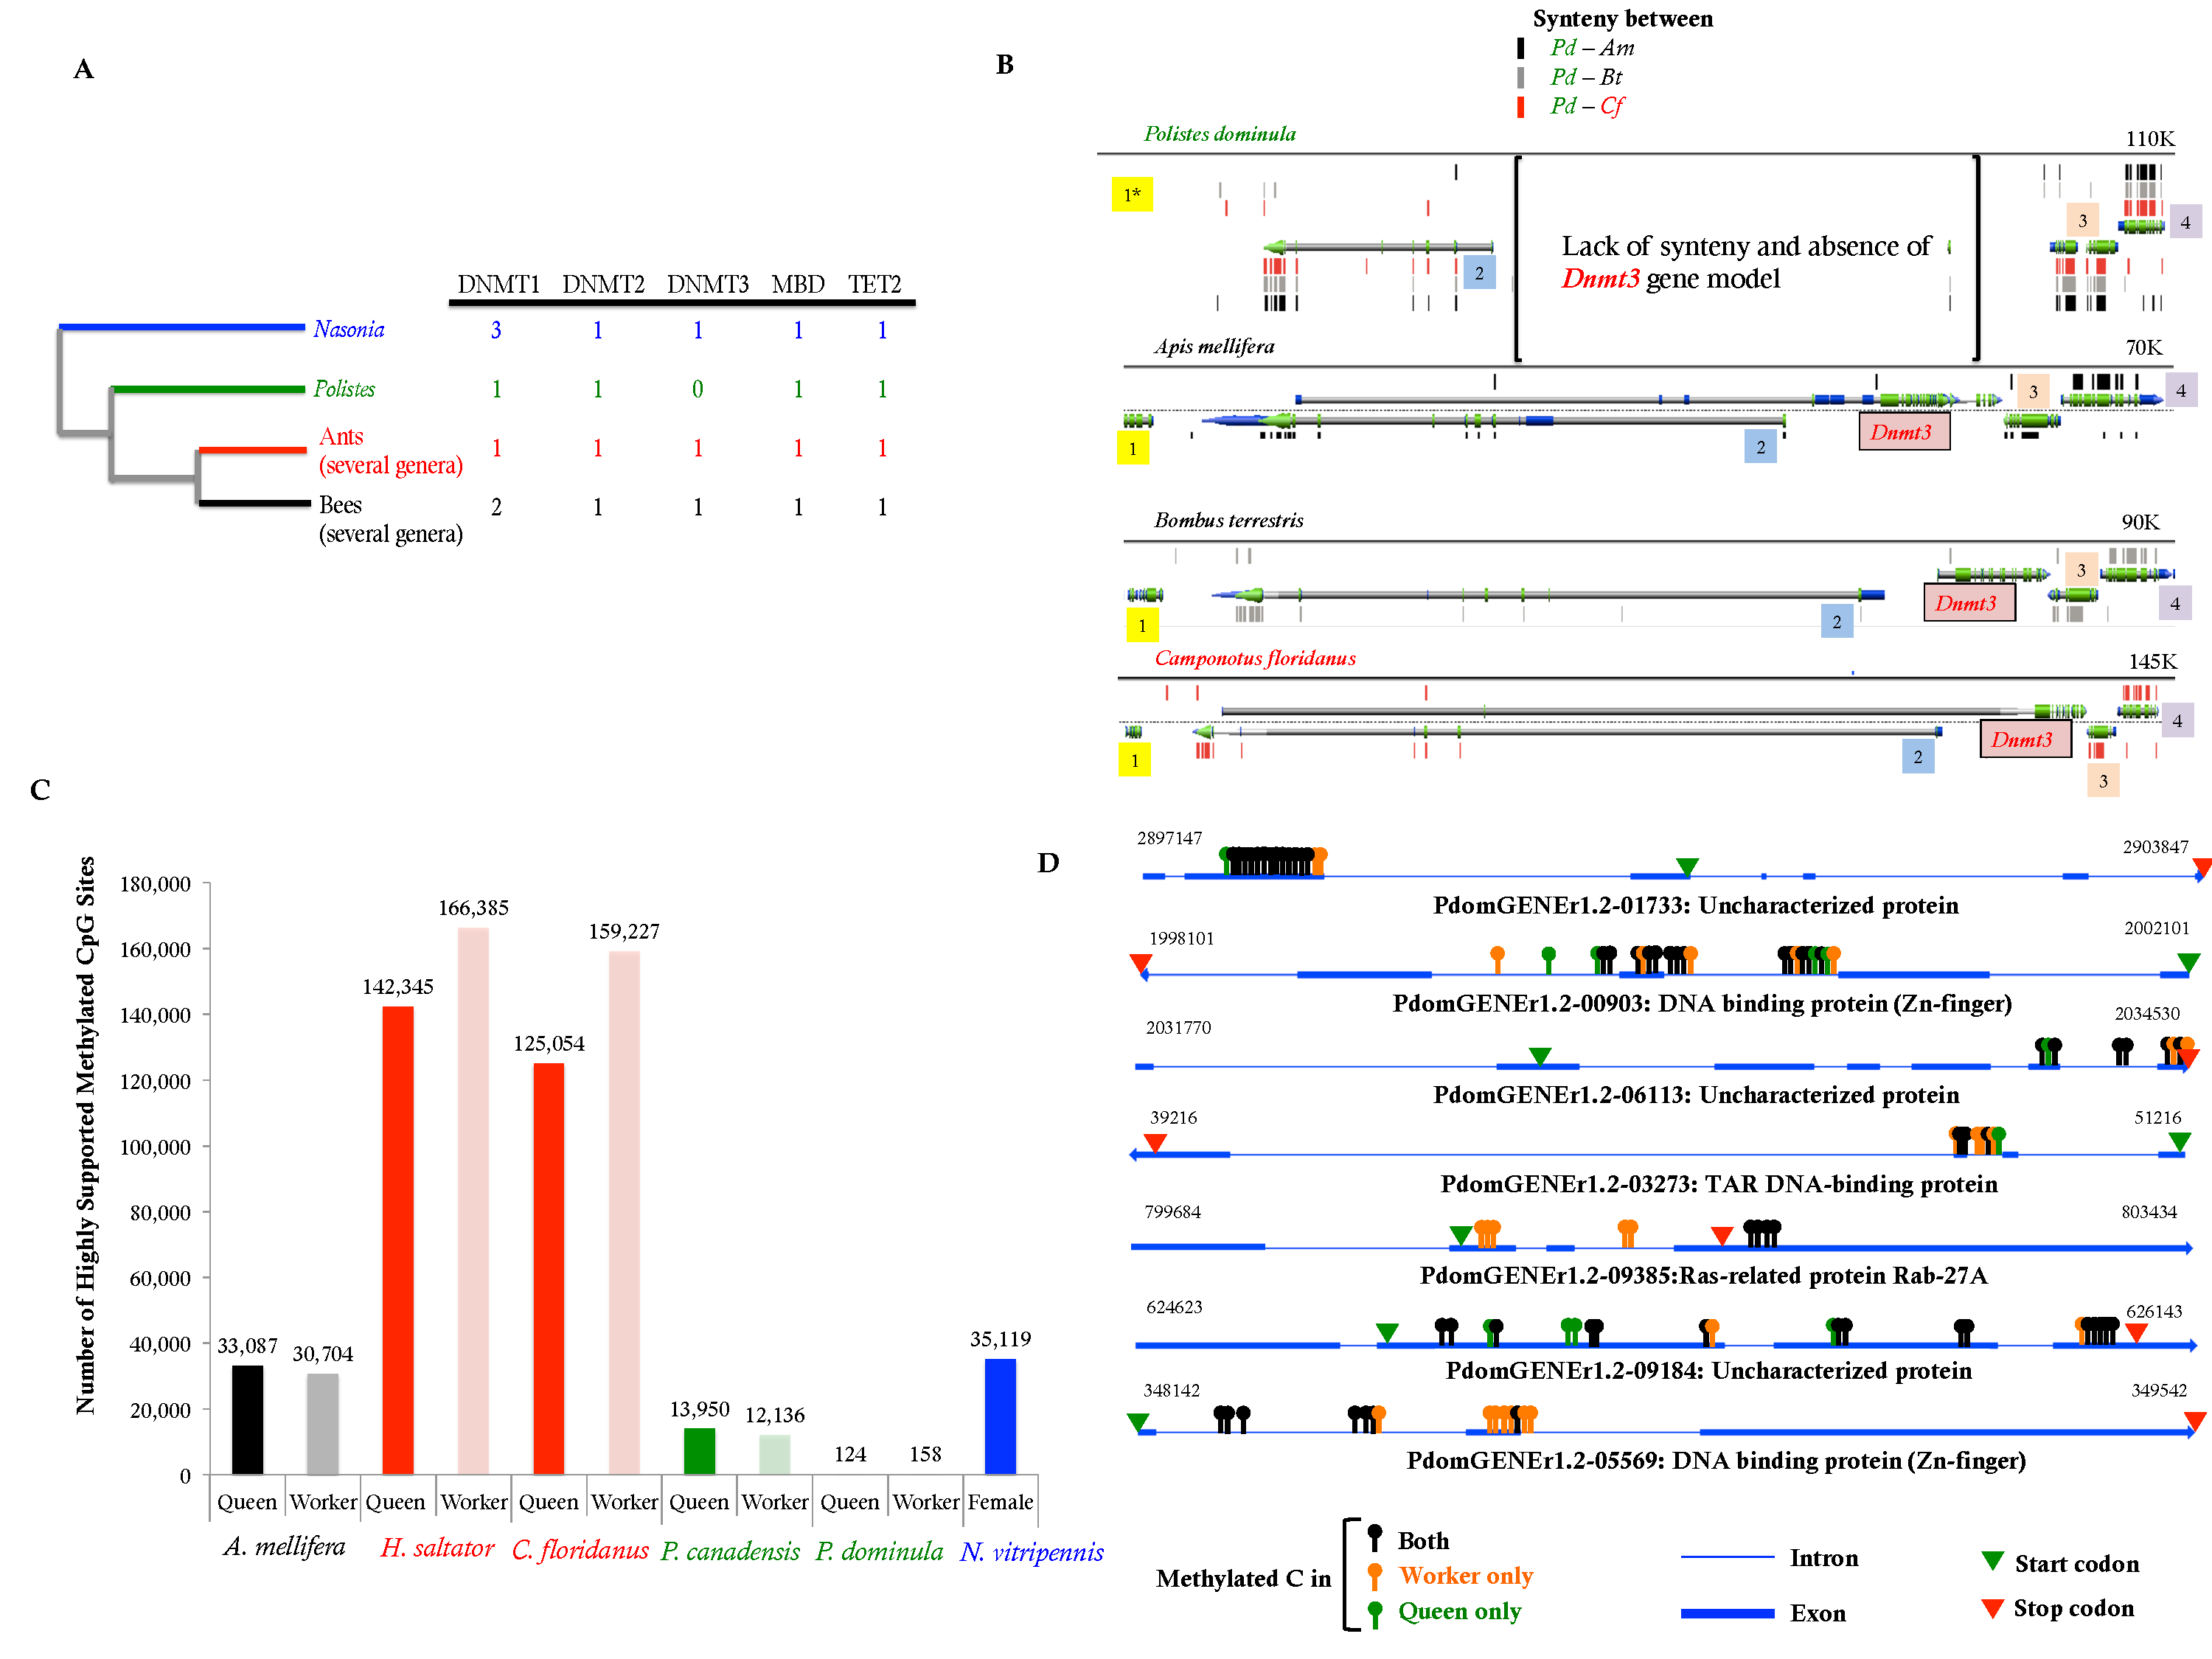
\includegraphics[width=8in]{Assets/Graphics/Pdom/figure-3}
\centering
\caption{~}
\label{Fig:Pdom3}
\end{sidewaysfigure}
